% Drawing 146/07-3 -- folder 146, batch 07, archive page 126 (PDF page 127).
% Transcription: tableau de graphes, une ligne par type $(g,\nu)$, avec à droite de chaque ligne un nombre qui est vraisemblablement la dimension $3g-3+\nu$. Dans chaque ligne, les graphes MD du type sont dessinés (sommets marqués de leur genre quand il est non nul, arêtes libres en flèches sortantes), reliés par des flèches de spécialisation dirigées vers les graphes plus simples, certaines affectées d'une multiplicité ($2$, $3$). $(0,3)$ : un sommet à trois arêtes libres ; nombre $0$. $(0,4)$ : le sommet à quatre arêtes libres $\leftarrow$ deux sommets trivalents joints par une arête ; nombre $1$. $(0,5)$ : sommet à cinq arêtes libres $\leftarrow$ deux sommets $\xleftarrow{2}$ trois sommets en chaîne ; nombre $2$. $(0,6)$ : sommet à six arêtes libres, puis graphes à deux, trois et quatre sommets, dont une étoile à trois branches, avec flèches marquées $2$ et $3$ ; nombre $3$. $(1,1)$ : un sommet de genre $1$ à une arête libre $\leftarrow$ une boucle à une arête libre ; nombre $1$. $(1,2)$ : sommet de genre $1$ à deux arêtes libres, puis boucle à deux arêtes libres, sommet de genre $1$ relié à un sommet trivalent, deux sommets joints par une double arête, etc., flèche marquée $2$ ; nombre $2$. $(1,3)$ : diagramme analogue, plus touffu, aboutissant à un triangle à trois arêtes libres, flèches marquées $2$ et $3$ ; nombre $3$. $(2,0)$ : sommet de genre $2$ ; sommet de genre $1$ à une boucle ; deux sommets de genre $1$ joints par une arête ; sommet de genre $1$ relié à une boucle ; huit (deux boucles en un sommet) ; deux sommets joints par trois arêtes ; flèches marquées $2$, $3$ et une flèche marquée d'un signe peu lisible ; nombre $3$. $(2,1)$ : premiers graphes seulement, puis « ……… » ; nombre $4$.
% Kind: table of stable (MD) graphs by type (g, nu). Method 3 (encoded, rendered from the data). Status: partial.
% Notes: Encoded and rendered canonically, not traced: for each row the stable graphs of type (g, nu) with unlabelled legs are enumerated by program (comb.enumerate_stable) and compared with the number he draws. Counts agree for (0,3) 1, (0,4) 2, (0,5) 3, (0,6) 7, (1,1) 2, (1,2) 5, (2,0) 7 (the 7 strata of M2-bar) and, re-counted on the crop, (1,3) 11 (two of them overinked), which the program also finds; (2,1): 16 exist, he draws the first 3 (genus-2 vertex with a leg; genus-1 vertex with a loop and a leg; two genus-1 vertices joined by an edge, with the leg under a scribble) and breaks off with « ……… » -- those 3 are rendered (the earlier rendering had dropped the third). His number at the right of each row equals 3g - 3 + nu in every row (0,1,2,3,1,2,3,3,4). Labels at \small. Still differs, and why it stays partial: the specialisation arrows between graphs and their multiplicities (2, 3, one illegible sign) are NOT encoded, so the rendering shows the graphs, not the arrows, and its layout is canonical (vertices on a line), so it does not lay over the page. Redrawn 2026-11-09 (issue 128): to check again. 2026-11-13, Claude Opus 5.5, overlay check (issue 147): the rendering is canonical (method 3: each row's stable graphs enumerated and laid out on a line), so it does not lay over the page by design; its check is the enumeration, which still agrees with the counts he draws. Not compiled (no TeX in the session). Still differs, as before, and why it stays partial: the specialisation arrows between the graphs and their multiplicities (2, 3, one illegible sign) are not encoded, and the layout is not his.
% Coordinates: 1 unit = 1 mm = 1/100 of the crop width (bbox in page fractions: [0.08, 0.06, 0.9, 0.86]).
% Redrawn by Claude (claude-opus-5-5), issue #73, 2026-11-09; not checked by a human; not compiled (no TeX in the session).
% Checked by Claude (claude-opus-5-5) 2026-11-13 (issue #147): canonical rendering, not laid over the facsimile by design, enumeration re-checked; not compiled (no TeX in the session). Not checked by a human. Status: partial.
% Rights: reproduces part of the work -- behind RENDER_TRANSCRIPTS, never published by itself.
\documentclass[tikz,border=3pt]{standalone}
\usepackage{amsmath,amssymb}
\usetikzlibrary{patterns,arrows.meta}
\tikzset{pencil/.style={black!45}, struck/.style={black!35}, mark/.style={circle,draw,inner sep=1.3pt}, pt/.style={circle,fill,inner sep=0.9pt}, opt/.style={circle,draw,fill=white,inner sep=1.1pt}}
\begin{document}
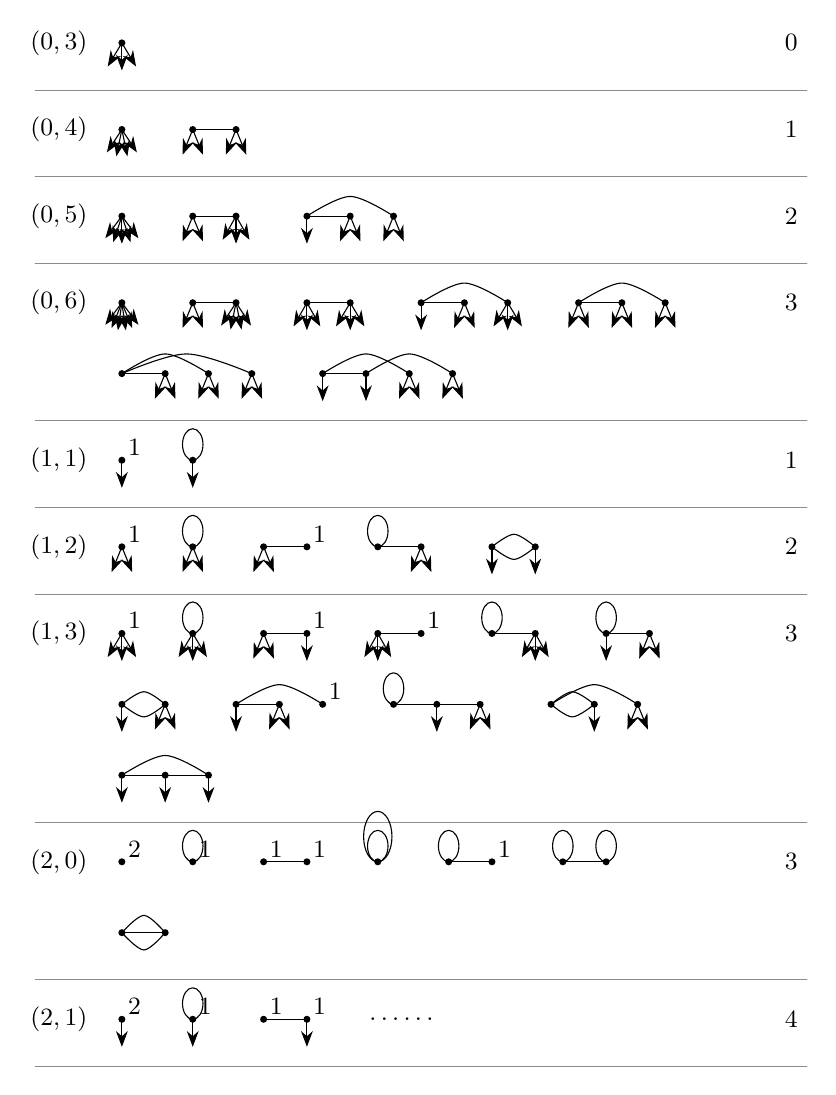
\begin{tikzpicture}[x=1mm,y=1mm,line cap=round,line join=round,font=\scriptsize]
\node[inner sep=1pt] at (4,-6) {\small $(0,3)$};
\node[inner sep=1pt] at (97,-6) {\small $0$};
\draw[-{Stealth[length=2mm]}] (12,-6) -- (13.8,-9);
\draw[-{Stealth[length=2mm]}] (12,-6) -- (12,-9.5);
\draw[-{Stealth[length=2mm]}] (12,-6) -- (10.2,-9);
\node[pt] at (12,-6) {};
\draw[pencil] (1,-12) -- (99,-12);
\node[inner sep=1pt] at (4,-17) {\small $(0,4)$};
\node[inner sep=1pt] at (97,-17) {\small $1$};
\draw[-{Stealth[length=2mm]}] (12,-17) -- (13.9,-19.9);
\draw[-{Stealth[length=2mm]}] (12,-17) -- (12.7,-20.4);
\draw[-{Stealth[length=2mm]}] (12,-17) -- (11.3,-20.4);
\draw[-{Stealth[length=2mm]}] (12,-17) -- (10.1,-19.9);
\node[pt] at (12,-17) {};
\draw (21,-17) -- (26.5,-17);
\draw[-{Stealth[length=2mm]}] (21,-17) -- (22.3,-20.2);
\draw[-{Stealth[length=2mm]}] (21,-17) -- (19.7,-20.2);
\node[pt] at (21,-17) {};
\draw[-{Stealth[length=2mm]}] (26.5,-17) -- (27.8,-20.2);
\draw[-{Stealth[length=2mm]}] (26.5,-17) -- (25.2,-20.2);
\node[pt] at (26.5,-17) {};
\draw[pencil] (1,-23) -- (99,-23);
\node[inner sep=1pt] at (4,-28) {\small $(0,5)$};
\node[inner sep=1pt] at (97,-28) {\small $2$};
\draw[-{Stealth[length=2mm]}] (12,-28) -- (14.1,-30.8);
\draw[-{Stealth[length=2mm]}] (12,-28) -- (13.1,-31.3);
\draw[-{Stealth[length=2mm]}] (12,-28) -- (12,-31.5);
\draw[-{Stealth[length=2mm]}] (12,-28) -- (10.9,-31.3);
\draw[-{Stealth[length=2mm]}] (12,-28) -- (9.9,-30.8);
\node[pt] at (12,-28) {};
\draw (21,-28) -- (26.5,-28);
\draw[-{Stealth[length=2mm]}] (21,-28) -- (22.3,-31.2);
\draw[-{Stealth[length=2mm]}] (21,-28) -- (19.7,-31.2);
\node[pt] at (21,-28) {};
\draw[-{Stealth[length=2mm]}] (26.5,-28) -- (28.2,-31);
\draw[-{Stealth[length=2mm]}] (26.5,-28) -- (26.5,-31.5);
\draw[-{Stealth[length=2mm]}] (26.5,-28) -- (24.8,-31);
\node[pt] at (26.5,-28) {};
\draw (35.5,-28) -- (41,-28);
\draw plot[smooth, tension=0.55] coordinates {(35.5,-28) (41,-25.5) (46.5,-28)};
\draw[-{Stealth[length=2mm]}] (35.5,-28) -- (35.5,-31.5);
\node[pt] at (35.5,-28) {};
\draw[-{Stealth[length=2mm]}] (41,-28) -- (42.3,-31.2);
\draw[-{Stealth[length=2mm]}] (41,-28) -- (39.7,-31.2);
\node[pt] at (41,-28) {};
\draw[-{Stealth[length=2mm]}] (46.5,-28) -- (47.8,-31.2);
\draw[-{Stealth[length=2mm]}] (46.5,-28) -- (45.2,-31.2);
\node[pt] at (46.5,-28) {};
\draw[pencil] (1,-34) -- (99,-34);
\node[inner sep=1pt] at (4,-39) {\small $(0,6)$};
\node[inner sep=1pt] at (97,-39) {\small $3$};
\draw[-{Stealth[length=2mm]}] (12,-39) -- (14.1,-41.8);
\draw[-{Stealth[length=2mm]}] (12,-39) -- (13.3,-42.2);
\draw[-{Stealth[length=2mm]}] (12,-39) -- (12.5,-42.5);
\draw[-{Stealth[length=2mm]}] (12,-39) -- (11.5,-42.5);
\draw[-{Stealth[length=2mm]}] (12,-39) -- (10.7,-42.2);
\draw[-{Stealth[length=2mm]}] (12,-39) -- (9.9,-41.8);
\node[pt] at (12,-39) {};
\draw (21,-39) -- (26.5,-39);
\draw[-{Stealth[length=2mm]}] (21,-39) -- (22.3,-42.2);
\draw[-{Stealth[length=2mm]}] (21,-39) -- (19.7,-42.2);
\node[pt] at (21,-39) {};
\draw[-{Stealth[length=2mm]}] (26.5,-39) -- (28.4,-41.9);
\draw[-{Stealth[length=2mm]}] (26.5,-39) -- (27.2,-42.4);
\draw[-{Stealth[length=2mm]}] (26.5,-39) -- (25.8,-42.4);
\draw[-{Stealth[length=2mm]}] (26.5,-39) -- (24.6,-41.9);
\node[pt] at (26.5,-39) {};
\draw (35.5,-39) -- (41,-39);
\draw[-{Stealth[length=2mm]}] (35.5,-39) -- (37.2,-42);
\draw[-{Stealth[length=2mm]}] (35.5,-39) -- (35.5,-42.5);
\draw[-{Stealth[length=2mm]}] (35.5,-39) -- (33.8,-42);
\node[pt] at (35.5,-39) {};
\draw[-{Stealth[length=2mm]}] (41,-39) -- (42.8,-42);
\draw[-{Stealth[length=2mm]}] (41,-39) -- (41,-42.5);
\draw[-{Stealth[length=2mm]}] (41,-39) -- (39.2,-42);
\node[pt] at (41,-39) {};
\draw (50,-39) -- (55.5,-39);
\draw plot[smooth, tension=0.55] coordinates {(50,-39) (55.5,-36.5) (61,-39)};
\draw[-{Stealth[length=2mm]}] (50,-39) -- (50,-42.5);
\node[pt] at (50,-39) {};
\draw[-{Stealth[length=2mm]}] (55.5,-39) -- (56.8,-42.2);
\draw[-{Stealth[length=2mm]}] (55.5,-39) -- (54.2,-42.2);
\node[pt] at (55.5,-39) {};
\draw[-{Stealth[length=2mm]}] (61,-39) -- (62.8,-42);
\draw[-{Stealth[length=2mm]}] (61,-39) -- (61,-42.5);
\draw[-{Stealth[length=2mm]}] (61,-39) -- (59.2,-42);
\node[pt] at (61,-39) {};
\draw (70,-39) -- (75.5,-39);
\draw plot[smooth, tension=0.55] coordinates {(70,-39) (75.5,-36.5) (81,-39)};
\draw[-{Stealth[length=2mm]}] (70,-39) -- (71.3,-42.2);
\draw[-{Stealth[length=2mm]}] (70,-39) -- (68.7,-42.2);
\node[pt] at (70,-39) {};
\draw[-{Stealth[length=2mm]}] (75.5,-39) -- (76.8,-42.2);
\draw[-{Stealth[length=2mm]}] (75.5,-39) -- (74.2,-42.2);
\node[pt] at (75.5,-39) {};
\draw[-{Stealth[length=2mm]}] (81,-39) -- (82.3,-42.2);
\draw[-{Stealth[length=2mm]}] (81,-39) -- (79.7,-42.2);
\node[pt] at (81,-39) {};
\draw (12,-48) -- (17.5,-48);
\draw plot[smooth, tension=0.55] coordinates {(12,-48) (17.5,-45.5) (23,-48)};
\draw plot[smooth, tension=0.55] coordinates {(12,-48) (20.2,-45.5) (28.5,-48)};
\node[pt] at (12,-48) {};
\draw[-{Stealth[length=2mm]}] (17.5,-48) -- (18.8,-51.2);
\draw[-{Stealth[length=2mm]}] (17.5,-48) -- (16.2,-51.2);
\node[pt] at (17.5,-48) {};
\draw[-{Stealth[length=2mm]}] (23,-48) -- (24.3,-51.2);
\draw[-{Stealth[length=2mm]}] (23,-48) -- (21.7,-51.2);
\node[pt] at (23,-48) {};
\draw[-{Stealth[length=2mm]}] (28.5,-48) -- (29.8,-51.2);
\draw[-{Stealth[length=2mm]}] (28.5,-48) -- (27.2,-51.2);
\node[pt] at (28.5,-48) {};
\draw (37.5,-48) -- (43,-48);
\draw plot[smooth, tension=0.55] coordinates {(37.5,-48) (43,-45.5) (48.5,-48)};
\draw plot[smooth, tension=0.55] coordinates {(43,-48) (48.5,-45.5) (54,-48)};
\draw[-{Stealth[length=2mm]}] (37.5,-48) -- (37.5,-51.5);
\node[pt] at (37.5,-48) {};
\draw[-{Stealth[length=2mm]}] (43,-48) -- (43,-51.5);
\node[pt] at (43,-48) {};
\draw[-{Stealth[length=2mm]}] (48.5,-48) -- (49.8,-51.2);
\draw[-{Stealth[length=2mm]}] (48.5,-48) -- (47.2,-51.2);
\node[pt] at (48.5,-48) {};
\draw[-{Stealth[length=2mm]}] (54,-48) -- (55.3,-51.2);
\draw[-{Stealth[length=2mm]}] (54,-48) -- (52.7,-51.2);
\node[pt] at (54,-48) {};
\draw[pencil] (1,-54) -- (99,-54);
\node[inner sep=1pt] at (4,-59) {\small $(1,1)$};
\node[inner sep=1pt] at (97,-59) {\small $1$};
\draw[-{Stealth[length=2mm]}] (12,-59) -- (12,-62.5);
\node[pt] at (12,-59) {};
\node[inner sep=1pt] at (13.6,-57.4) {\small $1$};
\draw (21,-57) ellipse[x radius=1.3, y radius=2];
\draw[-{Stealth[length=2mm]}] (21,-59) -- (21,-62.5);
\node[pt] at (21,-59) {};
\draw[pencil] (1,-65) -- (99,-65);
\node[inner sep=1pt] at (4,-70) {\small $(1,2)$};
\node[inner sep=1pt] at (97,-70) {\small $2$};
\draw[-{Stealth[length=2mm]}] (12,-70) -- (13.3,-73.2);
\draw[-{Stealth[length=2mm]}] (12,-70) -- (10.7,-73.2);
\node[pt] at (12,-70) {};
\node[inner sep=1pt] at (13.6,-68.4) {\small $1$};
\draw (21,-68) ellipse[x radius=1.3, y radius=2];
\draw[-{Stealth[length=2mm]}] (21,-70) -- (22.3,-73.2);
\draw[-{Stealth[length=2mm]}] (21,-70) -- (19.7,-73.2);
\node[pt] at (21,-70) {};
\draw (30,-70) -- (35.5,-70);
\draw[-{Stealth[length=2mm]}] (30,-70) -- (31.3,-73.2);
\draw[-{Stealth[length=2mm]}] (30,-70) -- (28.7,-73.2);
\node[pt] at (30,-70) {};
\node[pt] at (35.5,-70) {};
\node[inner sep=1pt] at (37.1,-68.4) {\small $1$};
\draw (44.5,-68) ellipse[x radius=1.3, y radius=2];
\draw (44.5,-70) -- (50,-70);
\node[pt] at (44.5,-70) {};
\draw[-{Stealth[length=2mm]}] (50,-70) -- (51.3,-73.2);
\draw[-{Stealth[length=2mm]}] (50,-70) -- (48.7,-73.2);
\node[pt] at (50,-70) {};
\draw plot[smooth, tension=0.55] coordinates {(59,-70) (61.8,-68.4) (64.5,-70)};
\draw plot[smooth, tension=0.55] coordinates {(59,-70) (61.8,-71.6) (64.5,-70)};
\draw[-{Stealth[length=2mm]}] (59,-70) -- (59,-73.5);
\node[pt] at (59,-70) {};
\draw[-{Stealth[length=2mm]}] (64.5,-70) -- (64.5,-73.5);
\node[pt] at (64.5,-70) {};
\draw[pencil] (1,-76) -- (99,-76);
\node[inner sep=1pt] at (4,-81) {\small $(1,3)$};
\node[inner sep=1pt] at (97,-81) {\small $3$};
\draw[-{Stealth[length=2mm]}] (12,-81) -- (13.8,-84);
\draw[-{Stealth[length=2mm]}] (12,-81) -- (12,-84.5);
\draw[-{Stealth[length=2mm]}] (12,-81) -- (10.2,-84);
\node[pt] at (12,-81) {};
\node[inner sep=1pt] at (13.6,-79.4) {\small $1$};
\draw (21,-79) ellipse[x radius=1.3, y radius=2];
\draw[-{Stealth[length=2mm]}] (21,-81) -- (22.8,-84);
\draw[-{Stealth[length=2mm]}] (21,-81) -- (21,-84.5);
\draw[-{Stealth[length=2mm]}] (21,-81) -- (19.2,-84);
\node[pt] at (21,-81) {};
\draw (30,-81) -- (35.5,-81);
\draw[-{Stealth[length=2mm]}] (30,-81) -- (31.3,-84.2);
\draw[-{Stealth[length=2mm]}] (30,-81) -- (28.7,-84.2);
\node[pt] at (30,-81) {};
\draw[-{Stealth[length=2mm]}] (35.5,-81) -- (35.5,-84.5);
\node[pt] at (35.5,-81) {};
\node[inner sep=1pt] at (37.1,-79.4) {\small $1$};
\draw (44.5,-81) -- (50,-81);
\draw[-{Stealth[length=2mm]}] (44.5,-81) -- (46.2,-84);
\draw[-{Stealth[length=2mm]}] (44.5,-81) -- (44.5,-84.5);
\draw[-{Stealth[length=2mm]}] (44.5,-81) -- (42.8,-84);
\node[pt] at (44.5,-81) {};
\node[pt] at (50,-81) {};
\node[inner sep=1pt] at (51.6,-79.4) {\small $1$};
\draw (59,-79) ellipse[x radius=1.3, y radius=2];
\draw (59,-81) -- (64.5,-81);
\node[pt] at (59,-81) {};
\draw[-{Stealth[length=2mm]}] (64.5,-81) -- (66.2,-84);
\draw[-{Stealth[length=2mm]}] (64.5,-81) -- (64.5,-84.5);
\draw[-{Stealth[length=2mm]}] (64.5,-81) -- (62.8,-84);
\node[pt] at (64.5,-81) {};
\draw (73.5,-79) ellipse[x radius=1.3, y radius=2];
\draw (73.5,-81) -- (79,-81);
\draw[-{Stealth[length=2mm]}] (73.5,-81) -- (73.5,-84.5);
\node[pt] at (73.5,-81) {};
\draw[-{Stealth[length=2mm]}] (79,-81) -- (80.3,-84.2);
\draw[-{Stealth[length=2mm]}] (79,-81) -- (77.7,-84.2);
\node[pt] at (79,-81) {};
\draw plot[smooth, tension=0.55] coordinates {(12,-90) (14.8,-88.4) (17.5,-90)};
\draw plot[smooth, tension=0.55] coordinates {(12,-90) (14.8,-91.6) (17.5,-90)};
\draw[-{Stealth[length=2mm]}] (12,-90) -- (12,-93.5);
\node[pt] at (12,-90) {};
\draw[-{Stealth[length=2mm]}] (17.5,-90) -- (18.8,-93.2);
\draw[-{Stealth[length=2mm]}] (17.5,-90) -- (16.2,-93.2);
\node[pt] at (17.5,-90) {};
\draw (26.5,-90) -- (32,-90);
\draw plot[smooth, tension=0.55] coordinates {(26.5,-90) (32,-87.5) (37.5,-90)};
\draw[-{Stealth[length=2mm]}] (26.5,-90) -- (26.5,-93.5);
\node[pt] at (26.5,-90) {};
\draw[-{Stealth[length=2mm]}] (32,-90) -- (33.3,-93.2);
\draw[-{Stealth[length=2mm]}] (32,-90) -- (30.7,-93.2);
\node[pt] at (32,-90) {};
\node[pt] at (37.5,-90) {};
\node[inner sep=1pt] at (39.1,-88.4) {\small $1$};
\draw (46.5,-88) ellipse[x radius=1.3, y radius=2];
\draw (46.5,-90) -- (52,-90);
\draw (52,-90) -- (57.5,-90);
\node[pt] at (46.5,-90) {};
\draw[-{Stealth[length=2mm]}] (52,-90) -- (52,-93.5);
\node[pt] at (52,-90) {};
\draw[-{Stealth[length=2mm]}] (57.5,-90) -- (58.8,-93.2);
\draw[-{Stealth[length=2mm]}] (57.5,-90) -- (56.2,-93.2);
\node[pt] at (57.5,-90) {};
\draw plot[smooth, tension=0.55] coordinates {(66.5,-90) (69.2,-88.4) (72,-90)};
\draw plot[smooth, tension=0.55] coordinates {(66.5,-90) (69.2,-91.6) (72,-90)};
\draw plot[smooth, tension=0.55] coordinates {(66.5,-90) (72,-87.5) (77.5,-90)};
\node[pt] at (66.5,-90) {};
\draw[-{Stealth[length=2mm]}] (72,-90) -- (72,-93.5);
\node[pt] at (72,-90) {};
\draw[-{Stealth[length=2mm]}] (77.5,-90) -- (78.8,-93.2);
\draw[-{Stealth[length=2mm]}] (77.5,-90) -- (76.2,-93.2);
\node[pt] at (77.5,-90) {};
\draw (12,-99) -- (17.5,-99);
\draw plot[smooth, tension=0.55] coordinates {(12,-99) (17.5,-96.5) (23,-99)};
\draw (17.5,-99) -- (23,-99);
\draw[-{Stealth[length=2mm]}] (12,-99) -- (12,-102.5);
\node[pt] at (12,-99) {};
\draw[-{Stealth[length=2mm]}] (17.5,-99) -- (17.5,-102.5);
\node[pt] at (17.5,-99) {};
\draw[-{Stealth[length=2mm]}] (23,-99) -- (23,-102.5);
\node[pt] at (23,-99) {};
\draw[pencil] (1,-105) -- (99,-105);
\node[inner sep=1pt] at (4,-110) {\small $(2,0)$};
\node[inner sep=1pt] at (97,-110) {\small $3$};
\node[pt] at (12,-110) {};
\node[inner sep=1pt] at (13.6,-108.4) {\small $2$};
\draw (21,-108) ellipse[x radius=1.3, y radius=2];
\node[pt] at (21,-110) {};
\node[inner sep=1pt] at (22.6,-108.4) {\small $1$};
\draw (30,-110) -- (35.5,-110);
\node[pt] at (30,-110) {};
\node[inner sep=1pt] at (31.6,-108.4) {\small $1$};
\node[pt] at (35.5,-110) {};
\node[inner sep=1pt] at (37.1,-108.4) {\small $1$};
\draw (44.5,-108) ellipse[x radius=1.3, y radius=2];
\draw (44.5,-106.8) ellipse[x radius=1.8, y radius=3.2];
\node[pt] at (44.5,-110) {};
\draw (53.5,-108) ellipse[x radius=1.3, y radius=2];
\draw (53.5,-110) -- (59,-110);
\node[pt] at (53.5,-110) {};
\node[pt] at (59,-110) {};
\node[inner sep=1pt] at (60.6,-108.4) {\small $1$};
\draw (68,-108) ellipse[x radius=1.3, y radius=2];
\draw (68,-110) -- (73.5,-110);
\draw (73.5,-108) ellipse[x radius=1.3, y radius=2];
\node[pt] at (68,-110) {};
\node[pt] at (73.5,-110) {};
\draw plot[smooth, tension=0.55] coordinates {(12,-119) (14.8,-116.8) (17.5,-119)};
\draw (12,-119) -- (17.5,-119);
\draw plot[smooth, tension=0.55] coordinates {(12,-119) (14.8,-121.2) (17.5,-119)};
\node[pt] at (12,-119) {};
\node[pt] at (17.5,-119) {};
\draw[pencil] (1,-125) -- (99,-125);
\node[inner sep=1pt] at (4,-130) {\small $(2,1)$};
\node[inner sep=1pt] at (97,-130) {\small $4$};
\draw[-{Stealth[length=2mm]}] (12,-130) -- (12,-133.5);
\node[pt] at (12,-130) {};
\node[inner sep=1pt] at (13.6,-128.4) {\small $2$};
\draw (21,-128) ellipse[x radius=1.3, y radius=2];
\draw[-{Stealth[length=2mm]}] (21,-130) -- (21,-133.5);
\node[pt] at (21,-130) {};
\node[inner sep=1pt] at (22.6,-128.4) {\small $1$};
\draw (30,-130) -- (35.5,-130);
\node[pt] at (30,-130) {};
\node[inner sep=1pt] at (31.6,-128.4) {\small $1$};
\draw[-{Stealth[length=2mm]}] (35.5,-130) -- (35.5,-133.5);
\node[pt] at (35.5,-130) {};
\node[inner sep=1pt] at (37.1,-128.4) {\small $1$};
\node[inner sep=1pt] at (47.5,-130) {\small $\ldots\ldots$};
\draw[pencil] (1,-136) -- (99,-136);
\end{tikzpicture}
\end{document}
